\documentclass[11pt,a4paper]{article}

%% Language and font encodings
\usepackage[utf8]{inputenc}
\usepackage[margin=1in]{geometry}
\usepackage{authblk}
\usepackage[style=apa]{biblatex}
\usepackage[american]{babel}
\usepackage[finalizecache,cachedir=.]{minted}
\usepackage{csquotes}
\DeclareLanguageMapping{american}{american-apa}
\bibliography{references.bib}

\usepackage{amsmath,amsfonts,amssymb,bm,bbm,amsthm}
\usepackage[colorinlistoftodos,textsize=small]{todonotes}
\usepackage{graphicx}
%\usepackage{breqn}
\usepackage{todonotes}
\usepackage{xcolor} % color math symbols, delete later
\usepackage{verbatim}
\newcommand\todoin[2][]{\todo[inline, caption={2do}, #1]{
	\begin{minipage}{\textwidth-4pt}#2\end{minipage}}
}
\usepackage{nicefrac}

\theoremstyle{definition} % no italiced theorem style
\newtheorem{prop}{Proposition}
\newtheorem{corr}{Corollary}[prop]
\newtheorem{lemma}[prop]{Lemma}

\newtheoremstyle{case}{}{}{}{}{}{:}{ }{}
\theoremstyle{case}
\newtheorem{case}{Case}

\usepackage[colorinlistoftodos,textsize=small]{todonotes}
\usepackage[colorlinks=true, allcolors=blue, bookmarks=false]{hyperref}


\newcommand{\iu}{{i\mkern1mu}}
\newcommand{\Lik}{\mathbb{L}}
\newcommand{\bx}{\bm{x}}
\newcommand{\by}{\bm{y}}
\newcommand{\bz}{\bm{z}}
\newcommand{\Reals}{\mathbb{R}}
\newcommand{\dx}[1]{\enspace \mathrm{d}{#1}}
\newcommand{\prior}[1]{\pi\left({#1}\right)}
\newcommand{\FGamma}[1]{\Gamma\left({#1}\right)}
\newcommand{\FBeta}[2]{\text{B}\left({#1},\ {#2}\right)}
\newcommand{\FHyperG}[1]{\, _2F_1\left({#1}\right)}
\newcommand{\FHyperGn}{\, _2F_1}
\newcommand{\mean}[1]{\overline{{#1}}}
\newcommand{\Lim}[1]{\raisebox{0.5ex}{\scalebox{0.8}{$\displaystyle \lim_{#1}\;$}}}
\newcommand{\BF}{\text{BF}}
\newcommand{\FHypGeo}[4]{\,_2F_1\left({#1};{#2};{#3};{#4}\right)}
\newcommand{\BetaBinom}[4]{\text{BB}\left(#1 \mid #2 ,\ #3 ,\ #4 \right)}

\newcommand{\dist}[1]{\pi\left(#1\right)}
\newcommand{\scaledDirichlet}[3]{\text{SD}\left(#1 \mid #2 ,\ #3\right)}
\newcommand{\simplex}[1]{\mathbb{S}^{#1}}
\newcommand{\Expectation}[1]{E\left[#1\right]}

\DeclareRobustCommand{\stirling}{\genfrac\{\}{0pt}{}}
\newcommand{\rstirling}[3]{\stirling{#1}{#2}_{#3}}
\newcommand{\bellnum}[1]{B_{#1}}
\newcommand{\rbellnum}[2]{B_{#1,\,#2}}
\newcommand{\setsize}[1]{|{#1}|}

\newcommand*\samethanks[1][\value{footnote}]{\footnotemark[#1]}

\newcommand{\numberthis}{\addtocounter{equation}{1}\tag{\theequation}}
\newcommand{\FD}[1]{\todo[inline, color=pink]{ \textbf{FD}: #1 }}
\newcommand{\DB}[1]{\todo[inline, color=orange]{ \textbf{DB}: #1 }}

\date{}
\title{Flexible Bayesian Multiple Comparison Adjustment}
\author[1]{Don van den Bergh\thanks{These authors contributed equally to this work.}}
\author[1]{Fabian Dablander\samethanks[1]}
\author[1]{Eric-Jan Wagenmakers}
\affil[1]{Department of Psychological Methods, University of Amsterdam}


\begin{document}
\maketitle

\section*{Outline}
\begin{enumerate}
    \item Introduction / Motivation
    \begin{itemize}
        \item Multiplicity adjustment for multiple comparisons
        \item Testing all possible hypotheses in an automatic manner (compared to frequentist setting: could sort the means and do $K - 1$ comparisons; errors might get exacerbated (one error early on puts lots of means into wrong partition); Rao's paradox (not reject the pairwise comparisons but would reject the joint); score-based likelihood approach (but computational explosion; K = 12 equals $>$ 4 million comparisons)
    \end{itemize}
    \item Comparison of Priors
    \begin{itemize}
        \item Introduce priors and classify them according to prediction rule and prior over partitions
        \item Priors are
        \begin{itemize}
            \item Dirichlet Process Prior \parencite{gopalan1998bayesian}. The problem with this prior is that it is not consistent \parencite{miller2013simple, miller2018mixture}
            \item Uniform Process \parencite{wallach2010alternative}. The problem is that this does not lead to an exchangeable partition.
            \item Beta-Binomial prior. Motivate through analogy with regression \parencite{scott2006exploration, scott2010bayes}.
        \end{itemize}
        \item Quantify the degree of multiplicity adjustment for pairwise comparisons by extending the trick in \textcite{scott2010bayes} and \textcite{li2016role}, apply to each prior
        \begin{itemize}
            \item Either compute $\frac{P(\mu_i = \mu_j | K)}{P(\mu_i = \mu_j | K + 1)}$ where $K$ indexes the number of groups; or compute the ratio of the probability that an additional group is equal to one of the other groups or not. Plot this ratio quantity as a function of the number of groups.
            \item Intuitively, as the number of groups grow, this ratio should grow as well (the new group mean is more likely to be equal to already observed group means). It is this shrinkage what gives multiplicity control.
            \item \textcite{scott2010bayes} study multiplicity adjustment by adding a bunch of variables that have zero effect and looking at how the posterior inclusion probabilities change. What would be the analogue for our multiple comparison case? Adding group means that are all equal?
            \item NB: the problem of multiplicity seems worse in variable selection; while there are more (pairwise) comparisons possible in ANOVA settings, one comparison gives information about all other comparisons involving that group.
        \end{itemize}
        \item Simulation study investigating (a) (in)consistency and (b) speed of convergence
    \end{itemize}
    \item Applications
    \begin{itemize}
        \item Proportions
        \item One-way ANOVA
        \item Variances
    \end{itemize}
    \item Conclusion
    \begin{itemize}
        \item Further research: species sampling models, mixture of finite mixtures
    \end{itemize}
\end{enumerate}

\section{Introduction}
Assessing the equality or inequality of groups is a key problem in science and applied settings. In experimental psychology, for example, memory researchers study whether a set of learning techniques differ in ... (CITE). In marketing, companies are interested in assessing the effect of distinct interventions (CITE). In political science, researchers ...

If a confirmatory hypothesis is lacking, a standard approach is to first test whether all groups are equal, and if not, engage in multiple post-hoc comparisons. A large swathe of multiple comparisons techniques to guard against inflated false positive errors exist in classical statistics dating back to the work of John Tukey and others \parencite[][]{rao2009multiple, benjamini2002john}. From a Bayesian perspective, the problem of multiple comparisons can be addressed by changing the model prior \parencite{jeffreys1961theory, westfall1997bayesian, berry1999bayesian}, which has found prominent application in variable selection for regression \parencite[e.g.,][]{scott2006exploration, scott2010bayes}. Here, we focus on a Bayesian multiplicity adjustment for testing the (in)equality of a set of groups by proposing a prior distribution over all possible partitions. This allows the researcher to explore the set of all possible equality and inequality relations among the groups while penalizing for multiple comparisons, a feat that is difficult to solve in a principled manner in classical statistics.

The first to propose a prior over all partitions to adjust for multiple hypotheses testing were, to our knowledge, \textcite{gopalan1998bayesian}, who suggested the Dirichlet Process (DP). As the authors admit this prior --- being governed by a single parameter --- lacks flexibility. Additionally, \textcite{miller2013simple} recently showed that the DP is inconsistent in selecting the correct number of partitions. The Pitman-Yor (PY) process is a generalization of the DP that increases flexibility \parencite{pitman1997two}. The PY yields similarly inconsistent inferences, however \parencite{miller2014inconsistency}. Moreover, both the DP and the PY assume a ``rich-get-richer'' structure which may be undesirable in the context of multiple comparisons.

To overcome these issues we propose a class of flexible Beta-binomial priors for Bayesian multiple comparison adjustment, inspired by recent work on variable selection in regression \parencite{scott2006exploration, scott2010bayes}. The paper is structured as follows. In Section \ref{sec:methodology}, we briefly review the Bayesian literature on multiple comparison, setup the problem we tackle, and describe the Polya urn scheme from which a number of priors can be derived that account for multiplicity. We characterize four such priors --- the DP, the PY, a uniform prior, and the Beta-binomial prior --- in Section \ref{sec:priors}. In Section \ref{sec:simulation-study} we present a simulation study comparing them. In Section \ref{sec:applications}, we illustrate our method on practical examples related to the comparison of means, variances, and proportions. Our method is available in the Julia package \textit{EqualitySelection}.


\section{Methodology} \label{sec:methodology}
\subsection{Problem Setup}
Our goal is to adjust for multiple comparisons in a flexible manner. Multiple comparisons are not a problem if a researcher wishes to compare only two hypothesis, denote them as $\mathcal{H}_0$ and $\mathcal{H}_1$. They way to do this is through use of the Bayes factor \parencite[e.g.,][]{kass1995bayes, ly2016harold}, which is given by:

\begin{equation}
    \text{BF}_{10} \equiv \frac{p(\mathcal{D} \mid \mathcal{H}_1)}{p(\mathcal{D} \mid \mathcal{H}_0)} \enspace ,
\end{equation}

where $\mathcal{D} = (Y_1, \ldots, Y_n)$ is the data. The Bayes factor does not depend on the number of hypotheses a researcher wishes to test. It is the same regardless of whether the researcher, say, is a neuroscientist and tests whether there is activity in one voxel or in $10,000$. A principled way to account for multiplicity is by adjusting the prior probability of the hypotheses \parencite[e.g.,][]{jeffreys1961theory, westfall1997bayesian}.

Suppose the researcher is interested in comparing $k$ groups, parameterized by $\theta = (\theta_1, \ldots, \theta_k)$. She is not only interested in whether all parameters are equal ($\mathcal{H}_0$) or whether they are unequal ($\mathcal{H}_1$), but also which pairs of parameters are equal or not. In the language of classical statistics, she is interested in post-hoc comparisons. We focus on a Bayesian solution to this problem in this paper. More specifically, going beyond classical tests, we consider the problem of assessing all possible equalities and inequalities between the groups. In general terms, the inference problem is:
\begin{align*}
    \theta &\sim \pi_{\theta}(.) \\
    \phi &\sim \pi_{\phi}(.) \\
    Y_i &\overset{i.i.d.}{\sim} P(Y_i \mid \theta, \phi)  \enspace ,
\end{align*}
where $\phi$ are nuisance parameters (in case they exist), such as the variances in an ANOVA, and $P$ is the likelihood. Using the posterior distribution of $\theta$, we can restate $\mathcal{H}_0$ as $p(\theta_1 = \theta_2 = \ldots = \theta_K \mid \mathcal{D})$ and $\mathcal{H}_1$ as $p(\theta_1 \neq \theta_2 \neq \ldots \neq \theta_k \mid \mathcal{D})$, but there are many more possible hypotheses, depending on the combination of equalities and inequalities. In the next section, we discuss and compare priors $\pi_{\theta}$ that allow for flexible multiplicity adjustment.


\subsection{Partitions}
The space of possible equality constraints for some parameter vector $\mathbf{\theta} = (\theta_1, \ldots, \theta_k)$ of size $k$ is equivalent to the partitions of that vector. For example, if $k = 3$ then the model that states $\theta_1 = \theta_2 \neq \theta_3$ is equivalent to the partition $\{\{\theta_1, \theta_2\}, \{\theta_3\}\}$. The space of possible models for $k = 5$ is shown in Figure~\ref{fig:partitions}.

\begin{figure}
    \centering
    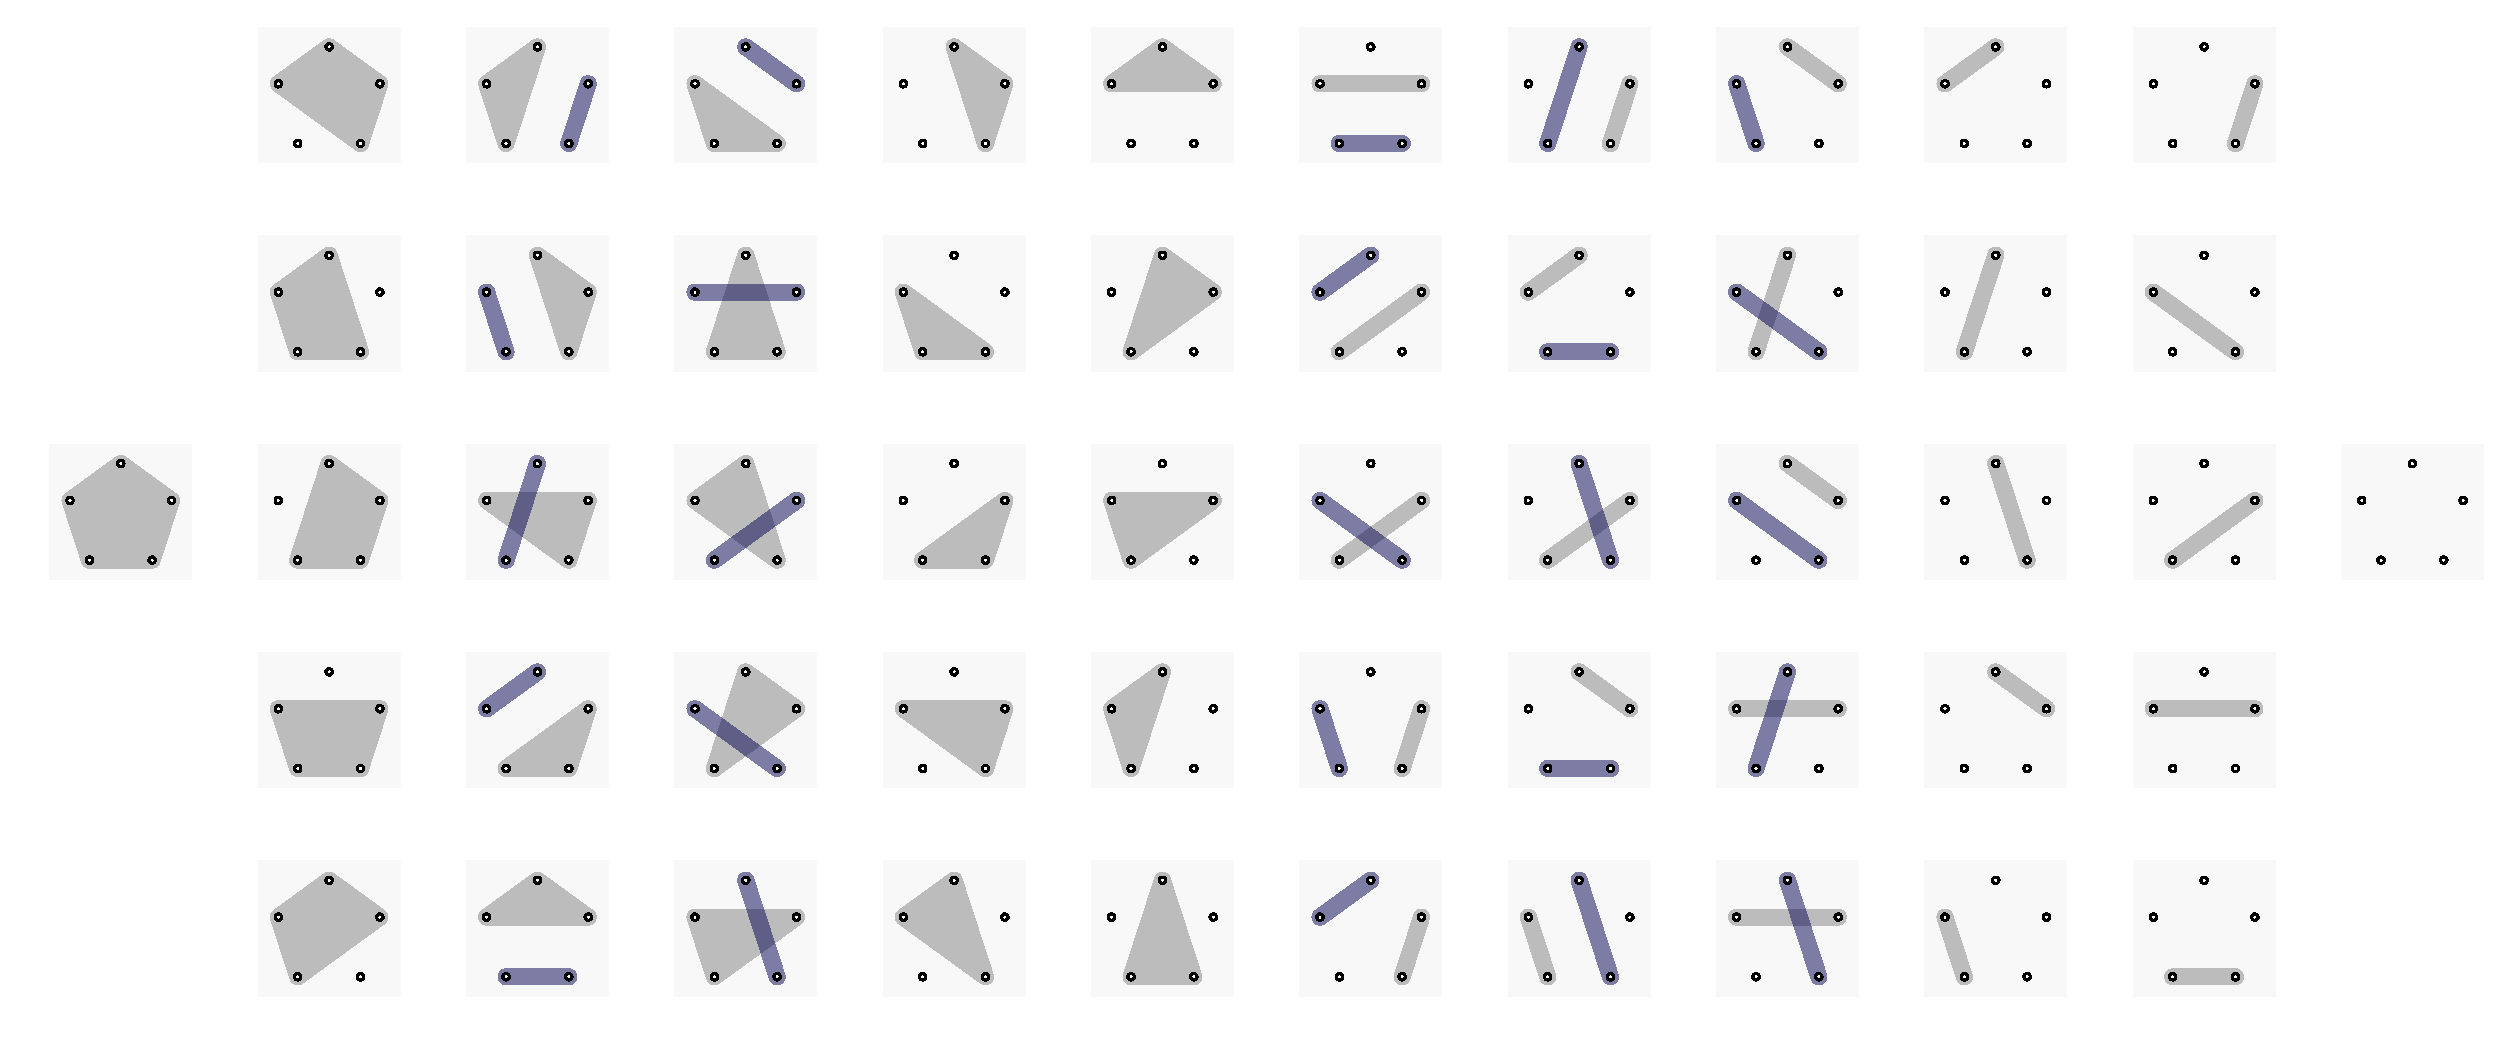
\includegraphics[width = \textwidth, keepaspectratio]{figures/modelspace_5_horizontal.pdf}
    \caption{All 52 possible models given $k = 5$, represented as partitions. Circles represent individual parameters and shaded regions indicate which parameters are equal.}
    % I know the ordering on wikipedia is better, but I didn't quite figure out how they did that
    \label{fig:partitions}
\end{figure}
%\DB{Do we want to follow APA7?}
%\FD{Only if it's nice. We're submitting to a statistics journal anyway.}

This equivalence is useful as partitions have been studied extensively in combinatorics. Given $k$ parameters, the number of partitions of size $j$ is given by the Stirling numbers of the second kind, denoted $\stirling{k}{j}$. The total number of partitions is given by the $k$\textsuperscript{th}-Bell number, which is defined as a sum over the Stirling numbers:
\begin{equation}
    \bellnum{k} = \sum_{i = 0}^k \stirling{k}{j} \enspace .
\end{equation}
The Bell numbers grow very quickly, with the number of partitions for a vector $\mathbf{\theta}$ of size 10 being $B_{10} =115975$. % B_10, not B_9 (21147)

The Stirling numbers and Bell numbers can be generalized to the $r$-Stirling \parencite{broder1984r} and $r$-Bell numbers \parencite{mezo2011r}. These generalizations help to construct conditional distributions, as will be shown later. The $r$-Stirling numbers $\rstirling{k}{j}{r}$ give the number of partitions of size $j$ given a $k$ parameters such that the first $r$ parameters are all in distinct subsets. The $r$-Bell numbers give the total number of partitions given $k$ parameters where the first $r$ parameters are in distinct subsets. Specifically, we have
\begin{align}
    \rstirling{k}{j}{r} &= \sum_{i=0}^k \binom{k}{i}\stirling{i}{j}r^{k-i}\\
    \rbellnum{k}{r} &= \sum_{i=0}^k \rstirling{k+r}{i+r}{r} \enspace .
\end{align}
Note that $\rstirling{k}{j}{1} = \stirling{k}{j}$ and that $\rbellnum{k}{0} = \bellnum{k}$. Both the $r$-Stirling and $r$-Bell are defined through recurrence relations, although explicit expressions exist which are easier to compute for large values. See \textcite{broder1984r} and \textcite{mezo2011r} for details.

\subsection{Urn Schemes}
Statistically, we represent the different partitions using an urn with $K$ different balls labeled 1 through $K$. For each parameter $\theta_i$, a ball $b_i$ is drawn from the urn with $b_i \in \{1,K\}$. If two drawn balls are equal, $b_i = b_j$, then the two parameters are assigned to the same subset of the partition, i.e., the two parameters, $\theta_i$ and $\theta_j$, are equal if $b_i = b_j$. Note that different draws from an urn can represent the same partition. For example, the draws $(1, 1, 2)$ and $(3, 3, 1)$ both represent the partition $\{\{\theta_1, \theta_2\}, \{\theta_3\}\}$. The prior distributions introduced in the next sections assign probabilities to the unique partitions. The prior probability for a particular draw can be obtained by dividing the probability of the corresponding partition by the total number of draws that correspond to that partition. The total number of draws that represent the same partition is given by $d!\binom{k}{d}$ where $d$ is the number of non-empty subsets of a particular draw. 

% not sure how to bring this up
Although the urn consists of $K$ different balls, the event of interest is the whether the next ball drawn equals one of the balls already drawn. In other words, whether an equality or inequality is introduced. This event reduces the urn to a P\'{o}lya urn. All prior distributions discussed below are related to the P\'{o}lya urn. Specifically, the joint prior distribution on $(\theta_1, \ldots, \theta_k)$ is characterized by a (generalized) P\'{o}lya urn such that:

\begin{equation} \label{eq:prediction-rule}
    P(\theta_k \mid \theta_1, \ldots, \theta_{k - 1}) = \begin{cases}
    \zeta_i & \text{with probability } P_{\pi} \\
    \theta_i^{\star} & \text{with probability }  1- P_{\pi} \enspace ,
    \end{cases} \numberthis
\end{equation}

where $\zeta_i$ denotes a new value for $\theta_i$ and $\theta_1 = \zeta_1$; and $\theta_i^{\star}$ denotes a value equal to any previously observed value. We characterize the priors we discuss in the next section in terms of (\ref{eq:prediction-rule}), which is known as a \textit{prediction rule} \parencite[e.g.,][]{ishwaran2001gibbs}; in terms of the induced prior over partitions; and in terms of their penalty for multiplicity.

%\FD{\textcite{ishwaran2001gibbs} might be useful, they use Polya Urns to derive a Gibbs sampler. They say it can be used for the Dirichlet process, but also for \textit{any} prior with known \textit{prediction rule}, which is defined as $P(Y_{n+1} \mid Y_1, \ldots, Y_n)$. I think this is a useful description which allows us to distinguish between several priors (Dirichlet, Pittman-Yor, Beta-binomial, etc.). Maybe note this here and then we refer to the next sections, in which we discuss the priors in slightly more detail?}
% We want to make inference over all possible partitions of some population parameter vector $\mathbf{\theta} = (\theta_1, \ldots, \theta_k)$ of size $k$. Each such partition corresponds do one particular hypothesis. The number of partitions $k$ is given by the Bell number

% \begin{equation}
%     B_{k + 1} = \sum_{i = 0}^k {k \choose i} B_k \enspace .
% \end{equation}

% The Bell numbers grow very quickly, with the number of partitions for a vector $\mathbf{\theta}$ of size 10 being 21147.


\section{Priors} \label{sec:priors}
Let $\mathbf{\theta^{\star}} = (\theta^{\star}_1, \ldots, \theta^{\star}_m)$ denote the vector of unique population parameters out of $\theta = (\theta_1, \ldots, \theta_k)$ and denote the number of repeats of $\theta^{\star}_j$ as $n^{\star}_j$. Let $\rho$ denote a partition and $|\rho|$ its size. For example, if $\rho = \{\{\theta_1, \theta_2\}, \{\theta_3\}\}$, then $|\rho| = 2$. In the next sections, we discuss and contrast a number of priors.

\subsection{Dirichlet Process Prior}
The Dirichlet Process is a stochastic process whose sample paths are distributions \parencite{ferguson1973bayesian}. It can be understood as the infinite-dimensional generalization of the Dirichlet distribution \parencite[e.g.,][]{teh2010dirichlet}, which makes it popular for mixture modeling \parencite{rasmussen1999infinite}. Our modeling approach is similar to mixture modeling, except that we do not cluster data but parameters; a cluster corresponds to a partition. The prediction rule of the DP is given by \parencite[e.g.,][]{ishwaran2001gibbs, blackwell1973ferguson}:

\iffalse
\begin{equation}
    P(\theta_K \mid \theta_1, \ldots, \theta_{K - 1}) = \frac{\alpha}{\alpha + K - 1} \mathcal{G}_0 + \sum^{m_K}_{j = 1} \frac{n^{\star}_{j, K}}{\alpha + K - 1} \delta_{\theta^{\star}_{j, K}}(.) \enspace .
\end{equation}
\fi

\begin{equation} \label{eq:prediction-rule}
    \theta_k \mid \theta_1, \ldots, \theta_{k - 1} \sim \begin{cases}
    \mathcal{G} & \text{with probability } \frac{\alpha}{\alpha + k - 1} \\
    \text{Categorical}\left(\theta_1^{\star}, \ldots, \theta_m^{\star} \mid n^{\star}_1, \ldots, n^{\star}_m\right) & \text{else} \enspace .
    \end{cases} \numberthis
\end{equation}

In other words, we draw a new value for $\theta_k$ from the Dirichlet process with probability $\nicefrac{\alpha}{\alpha + k - 1}$, or else set it to a previously observed value. The particular value $\theta^{\star}_j$ the parameter $\theta_k$ is set to is proportional to the number of times $\theta^{\star}_j$ was observed previously, given by $n^{\star}_j$, resulting in the well-known ``rich-get-richer'' property \parencite[e.g.,][]{teh2010dirichlet}.

We can integrate out $\mathcal{G}$ to get a prior distribution over partitions --- the so-called \textit{Chinese Restaurant Process} \parencite[e.g.,][]{teh2010dirichlet}. The prior on the partitions $\rho$ is:

\begin{equation}
    \pi(\rho \mid \alpha) = \frac{\alpha^{|\rho|}\Gamma(\alpha)}{\Gamma(n + \alpha)} \prod_{c \in \rho} \Gamma(|c|) \enspace ,
\end{equation}

where $c$ is an element of $\rho$, and $|c|$ is its size.

Observe that while the prediction rule features the infinite-dimensional object $\mathcal{G}$, the prior over partitions results from integrating it out. Hence the nonparametric model (in which the number of parameters is not fixed) implies a parametric model (in which the number of parameters is fixed) for the partitions \parencite{quintana2006predictive}. This makes it usable for our purposes, where we have a fixed number of parameters.

The Dirichlet process has a single parameter $\alpha$, which renders it inflexible \parencite{gopalan1998bayesian}. The Pitman-Yor process generalizes the DP \parencite{pitman1997two}, but it, too, assumes a ``rich-get-richer'' structure which may be undesirable. Both the DP and the PY are instances of so-called \textit{species-sampling models} (SSM), which are a general class of nonparametric models \parencite[e.g.,][]{lee2013defining, ishwaran2003generalized, pitman1996some}. To keep this paper contained, however, we focus on the DP as the only example of a nonparametric model.

\subsection{Uniform Prior}
\FD{The paper by \textcite{wallach2010alternative} seems extremely relevant here. The define the uniform process as having a prediction rule that is uniform over the already existing partitions ... so not quite the same. How is it related to what we do here? Actually, they show that the expected number of clusters of size $M$ is a constant, so it seems to be exactly what we do. Interestingly, the uniform process is not exchangeable. Also, it seems to me that it will not penalize multiplicity.}
For completion, we derive a prior that is uniform over the space of partitions. The probability mass function is straightforward. All valid configurations of size $k$ have probability $1 / \bellnum{k}$.


% \begin{align*}
%     \prior{b_1 = k} &= \frac{1}{k}, \\
%     \prior{b_i = k\mid \{b_1,\dots,b_{i-1}\}} &\propto 
%     \begin{cases}
%         \rbellnum{k - i - 1}{s_i} &\text{if $k\in\{b_1,\dots,b_{i-1}\}$}\\
%         \frac{1}{k - s_i}\rbellnum{k - i - 1}{s_i + 1}\quad &\text{if $k\notin\{b_1,\dots,b_{i-1}\}$}
%     \end{cases}
% \end{align*}

\begin{equation}
    \prior{\theta_i \mid \theta_1, \ldots, \theta_{i - 1}} = \begin{cases}
    \zeta_i & \text{with probability proportional to } \rbellnum{k - i - 1}{s_i + 1} \\
    \theta_i^\ast & \text{with probability proportional to }  \rbellnum{k - i - 1}{s_i} \enspace
    \end{cases} \numberthis
\end{equation}


where $s_i = \setsize{\{\theta_1, \ldots, \theta_{i - 1}\}}$, the number of distinct elements in $\{\theta_1, \ldots, \theta_{i - 1}\}$. For the first value $\theta_1$, the drawn value is irrelevant as it does not introduce an (in)equality. For the second draw we consider two cases. First, the probability of drawing a new value, $\theta_2 \neq \theta_1$ is proportional to the number of models where the first two elements are in distinct subsets, $\rbellnum{k - 2}{2}$. This probability of sampling a particular  is uniformly divided over the the possible labels, so to obtain the probability for a particular we divide by $k - s_i$. Second, the probability of drawing an old label, $\theta_2 = \theta_1$, is proportional to the number of models where the first element is in a distinct subset.

\subsection{Beta-Binomial Prior}
\FD{Need to write down the prediction rule and the expected size of unique clusters $m$. So write it as two steps: first either old or new; second as a Dirichlet where the weights a given by the Bell numbers (for sampling an old one).}
Here we briefly introduce the Beta-Binomial model prior, its properties, and how we can apply use it to the space of equality constraints. The Beta-Binomial model prior is often-used in linear regression when doing stochastic search variable selection \parencite[SSVS;][]{george1993variable} or Bayesian Model Averaging \parencite[BMA;][]{hinne2020conceptual, hoeting1999bayesian}. It states that the prior probability of including $j$ predictors out of a total of $k$ predictions is given by
\begin{equation}
    \BetaBinom{j}{k}{\alpha}{\beta} = \binom{k}{j} \frac{\FBeta{j + \alpha}{k - j + \beta}}{\FBeta{\alpha}{\beta}} \enspace ,
\end{equation}
where $\alpha$ and $\beta$ are hyperparameters. The prior probability of a particular model is obtained by dividing by the number of ways $j$ out of $k$ predictors can be included: $\BetaBinom{j}{k}{\alpha}{\beta} / \binom{k}{j}$. The advantage of the Beta-Binomial distribution is that it introduce a penalty for including additional predictors and in that way introduces a correction for multiplicity \parencite{scott2010bayes}.

In the space of equality constraints, we consider the number of inequality constraints and use the Beta-Binomial prior to introduce a penalty for each additional inequality among the variables considered. This yields the following prior distribution over the number of included inequalities: $\BetaBinom{j}{k-1}{\alpha}{\beta}$. To obtain the prior probability for a particular model, divide by the number of ways we can choose $j$ out of $k-1$ inequalities and obtain $\BetaBinom{j}{k-1}{\alpha}{\beta} / \stirling{k}{k-j}$.
% TODO DB: rewrite this in terms of a partition 


The probability for the prediction rule for the Beta-Binomial prior is given by:

\begin{equation}
    P(\zeta_i) = \frac{
        \sum_{j=1}^k \BetaBinom{j}{k}{\alpha}{\beta} \rstirling{k-j-s_i-1}{k-j+1}{s_i + 1}
    }{
        s_i \sum_{j=1}^k \BetaBinom{j}{k}{\alpha}{\beta} \rstirling{k-j-s_i-2}{k-j+1}{s_i    } +
          \sum_{j=1}^k \BetaBinom{j}{k}{\alpha}{\beta} \rstirling{k-j-s_i-1}{k-j+1}{s_i + 1}
    }
\end{equation}
The $r$-Stirling number in the numerator counts the number of models with $j$ equalities if $\theta_i$ is a new value. Next, this is multiplied by the probability of including $j$ equalities. This is summed for all possible numbers of equalities. 
The first sum in the denominator does the same, assuming that $theta_i$ is a value in $\{\theta_1, \dots, \theta_{i-1}\}$. With probability $1 - P(\zeta_i)$ we have that $\theta_i$ is equal to one of the previously drawn parameters. This draw is uniform over the possible models, that is, conditional on drawing a previous value the probability of $\theta_i = \theta_j$ is proportional to $\bellnum{k-j-1}{s_i}$.

\begin{figure}
    \centering
    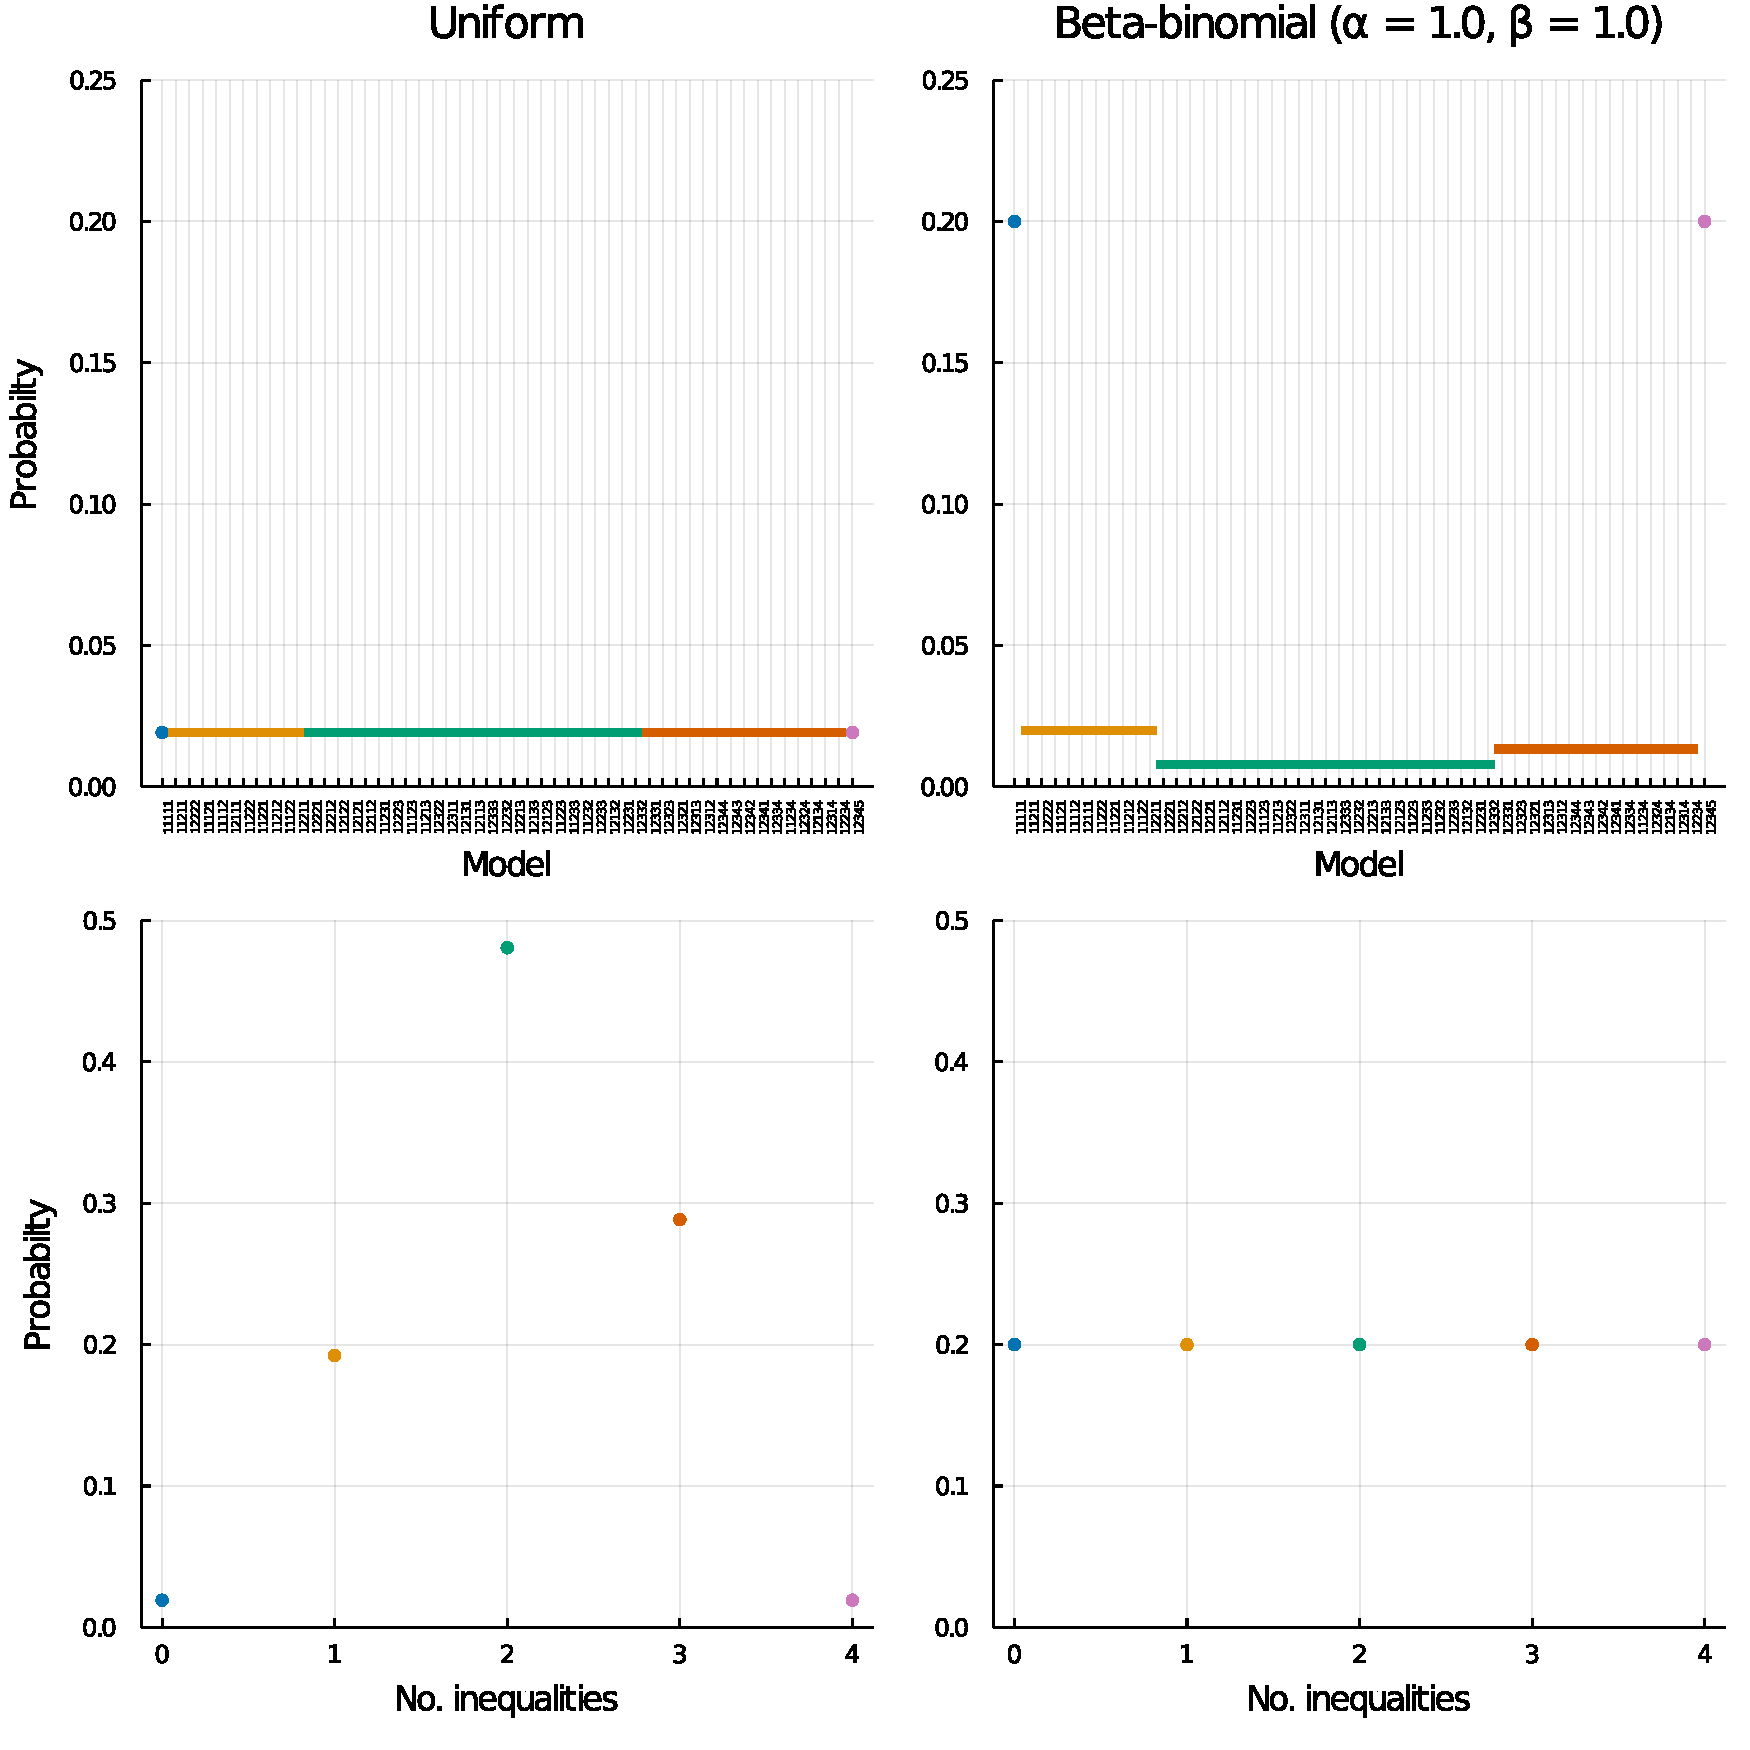
\includegraphics[width = \textwidth]{figures/prior_5.pdf}
    \caption{%
    Properties of the uniform prior (left column) and beta-binomial prior (right column) for $k = 5$. The top row shows the prior model probabilities whereas the bottom row shows the prior probability of a particular number of inequalities. While the uniform prior is uniform over the models, it is not uniform over the number of inequalities. In contrast, the beta-binomial prior is uniform over the number of inequalities but not uniform over the models. In all figures, colors correspond to the number of inequalities in the model. The x-axis in the top row displays the models with an indicator notation, for example, `11111' denotes the model where all parameters are equal.
    }
    \label{fig:my_label}
\end{figure}
\FD{Looks great! Maybe we can make the dots bigger so one sees the colour better? We also need to show the DP. Change x-axis to have images from Figure 1.}

\subsection{Comparison of Priors}

\begin{itemize}
    \item \textcolor{red}{NEED SCOTT \& BERGER PLOT FOR THE THREE PRIORS}
    \item \textcolor{red}{NEED A PLOT SHOWING THE EXPECTED NUMBER OF CLUSTERS}
\end{itemize}



\section{Simulation Study} \label{sec:simulation-study}
\subsection{Convergence Rate}
\FD{Plot: For each prior, simulate from true model and plot posterior probability as sample size increases. Ideally, we see that DP is not consistent.}
\textcite{chen1995optimal} showed that the optimal rate of convergence in the finite mixture problem when the number of components are unknown is $n^{-\frac{1}{4}}$ (with knowledge of the components, the rate can be $\sqrt{n}$). \textcite{ishwaran2001bayesian} show that a Bayesian estimation method is consistent and achieves the $n^{-\frac{1}{4}}$ convergence rate in finite mixtures with the number of components unknown.

\textcite{miller2014inconsistency} argue that nonparametric clustering using a large class of models is inconsistent; see also \textcite{miller2013simple}, for an example. \textcite{miller2018mixture} therefore suggest mixture models with a prior on the number of components with support $\mathbb{N}$ instead of using a nonparametric approach. See also \textcite{green2001modelling} for a comparison of the two approaches.

\section{Application} \label{sec:applications}
\subsection{Testing Proportions}
\subsection{Testing Means}
\subsection{Testing Variances}

\section{Discussion} \label{sec:discussion}
\textcite{kim2009spiked} combine a spike at zero with a DPP. \textcite{curtis2011bayesian} also use a DPP to combine clustering o highly correlated predictors in linear regression with variable selection. \textcite{canale2017pitman} focus on the Pitman-Yor process, which is a generalization of the DPP. \textcite{lu2018reducing} study a powered Chinese restaurant process. \textcite{miller2015microclustering} study a microclustering property, for which the number of data points in a cluster does not grow linearly with the total number of data points (which is assumed by the DP, PY, etc.)

We focused on independent groups, but one could model dependencies using the distance CRP \parencite{blei2011distance}.

%\textit{This paper grew out of our response to an anonymous reviewer of another paper.}

\printbibliography
\end{document}